\newpage
\section{Classification of Self-Adaptive Systems}
\label{ch:SASClassification}

There are different approaches on how to classify and describe \acrshort{sas} which all focus on different usages.
The three approaches that will be highlighted by this section are:
\begin{itemize}[nosep]
    \item FORMS \cite*{FORMS}
    \item Berns' and Ghosh's definition of self-* properties \cite*{DissectingSelfProperties}
    \item Krupitzer's et al. taxonomy for \acrshort{sas} \cite*{SurveyOnEngineeringApproaches}
\end{itemize} 
These approaches contain ideas that will be used to construct the classification for
\acrshort{oa} for \acrshort{sas} in the next chapter.

\begin{figure*}[b!]
    \centering
    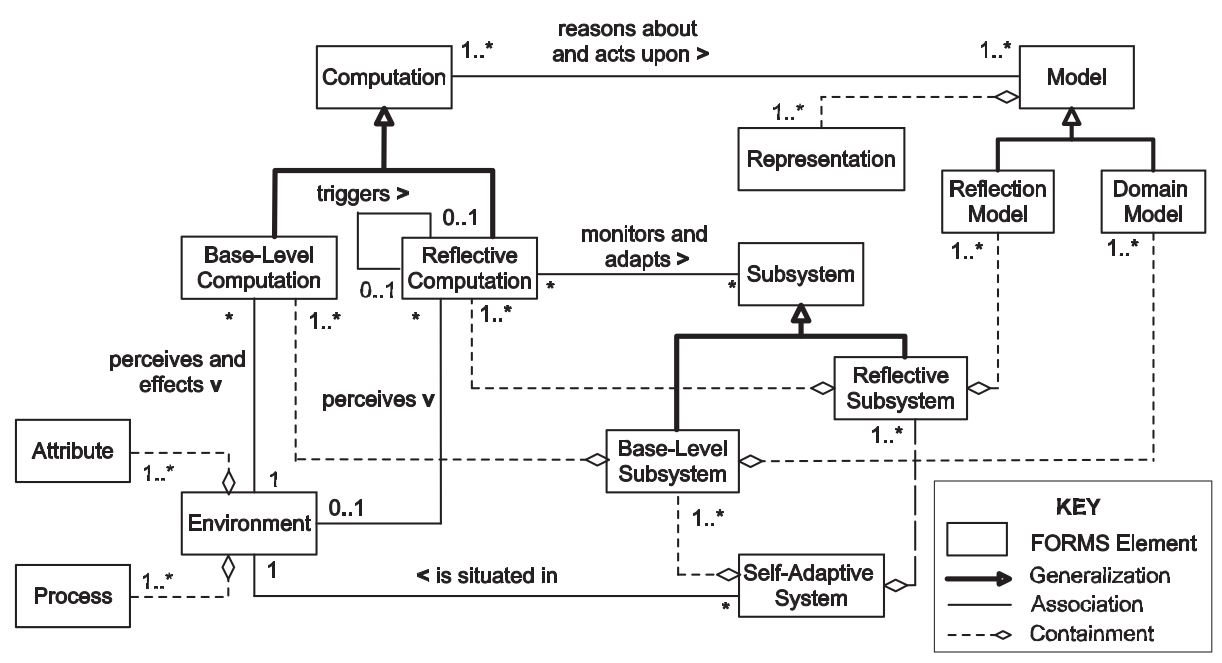
\includegraphics[width=\textwidth]{images/FORMS.png}
    \caption{FORMS primitives \cite*{FORMS}}
    \label{fig:FORMS}
\end{figure*}

\noindent With FORMS Weyns et al. propose a formal reference model for describing \acrshort{sas} \cite{FORMS}.
The goal of FORMS is to provide a well defined basis for talking and reasoning about \acrshort{sas}.
This is achieved by constructing \acrshort{sas} from a set of primitives which are defined in Z notation.
Z notation is used for formal specifications and is based upon Zermelo-Fraenkel set theory.
It is mathematically well-defined and often used to describe software systems.

\noindent Figure \ref{fig:FORMS} shows all the primitives used by FORMS and their relationships.
The \acrshort{sas} is split into different layers of subsystems.
Base-level refers to subsystems on the bottom most layer of the system.
Subsystems in layers above the base-level layer are called reflective.
Reflection refers to the ability of a system to inspect and change itself.

\noindent Each subsystem consists of two parts: its computation and its model.
Base-level subsystems have domain models which contain data about the environment.
In addition to that, reflective subsystems also have a reflection model which contains data about the system itself.
While base-level subsystems can use their computation to affect the environment,
reflective subsystems can affect the subsystems in the layer below themselves.

\noindent This approach can be understood with the example of a robot that uses motorized wheels
and some sensors to observe its environment.
The motor control software used by the robot would be placed in the base-level layers.
The sensors would be placed in the base-level layer as well.
These components are responsible for observing the environment and interacting with it.
On top of the base-level layer the robot might use a reflective layer which changes how the wheels are operated
based on the current weather conditions that it observes.
The top layer of the robots software could be an automatic updater 
which automatically updates the robots software to the latest version.
For this, the updater has to examine the robots software and modify it.
In other words, the updater is a reflective component.

\noindent The concept of different layers of reflection will be useful later to distinguish
\acrshort{oa} from \acrshort{sas}.

%% self-* properties
\begin{figure*}[t!]
    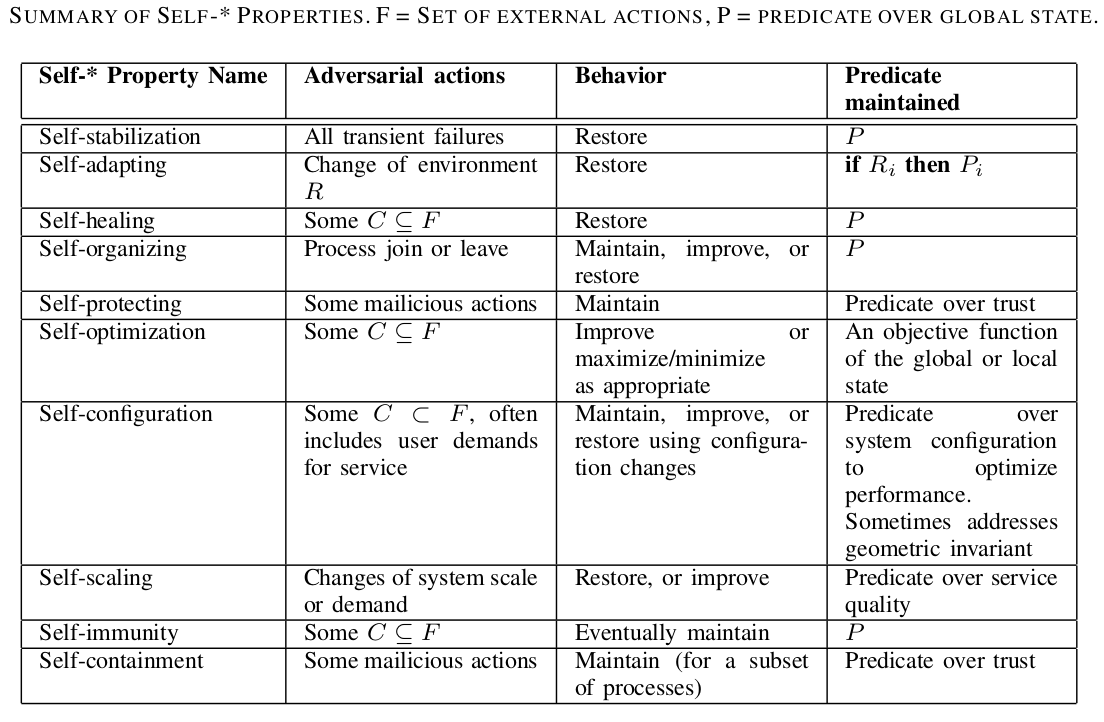
\includegraphics[width=\textwidth]{images/SelfProperties.png}
    \caption{self-* properties \cite*{DissectingSelfProperties}}
    \label{fig:SelfProperties}
\end{figure*}

\noindent Although some of the first papers on \acrshort{sas}, for example, 
"The Vision of Autonomic Computing" by Kephart and Chess \cite*{VisionOfAutonomicComputing} focused on self-adaptation,
there are other aspects of software systems that can benefit from the ideas introduced by \acrshort{sas}.
Berns and Ghosh identified and described such aspects which they call self-* properties \cite*{DissectingSelfProperties}.
They found the self-* properties that are depicted in Figure \ref{fig:SelfProperties}.

\noindent Berns and Ghosh describe \acrshort{sas} in terms of their interaction with their environment
and their reaction to external actions \cite*{DissectingSelfProperties}.
External actions are actions stemming from the systems environment which affect the system directly.
Safety predicates are used to describe goals of the system.
These external actions are called malicious if the intent of the action is the violation of a safety predicate.
A system also has a configuration which is the collection of its parameters.
Using these definitions, Berns and Ghosh describe their self-* properties in the following way:

\subparagraph*{Self-stabilization}
A system has the self-stabilization property if it can get from any starting configuration
to a configuration in which its safety predicates are fulfilled and stay in such a configuration afterwards.
In other words: The system can complete its starting procedure without requiring assistance.
\subparagraph*{Self-adapting}
A system is self-adapting (or managing) if it maintains, improves or restores safety predicates
without human intervention.
This definition matches the definition proposed by Kephart and Chess \cite*{VisionOfAutonomicComputing}
of systems which can autonomously manage themselves without human intervention.
\subparagraph*{Self-healing}
A system is self-healing if an external action can only cause a temporary violation of safety predicates.
This means that a self-healing system can recover from external actions on its own.
An example would be a system which can restart itself after a power outage.
\subparagraph*{Self-organizing}
A system is self-organizing if it maintains, improves or restores safety predicates after an external
action which involves processes joining or leaving the system. The recovery time per join or leave should be sublinear.
Peer-to-peer networks can be examples for self-organizing systems.
\subparagraph*{Self-protecting}
A system is self-protecting if it maintains one chosen safety predicate even when malicious external actions occur.
Meaning that a self-protecting system guarantees that it will never violate the chosen safety predicate.
A real world example for this would be a system which guarantees that it will not disclose personal data to unauthorized users.
\subparagraph*{Self-optimization}
When a system is self-optimizing, it can maximize or minimize the value of a utility function.
A system which starts and stops services based on demand to reduce energy usage is an example for a self-optimizing system.
\subparagraph*{Self-configuration}
A system possesses the self-configuration property if it can change its configuration to restore or improve a safety predicate.
\subparagraph*{Self-scaling}
A self-scaling system can maintain or improve a system property while an external action affects its scale.
This means that a system which regulates the number of instances of one of its services based, for example, on demand is self-scaling.
\subparagraph*{Self-immunity}
A system with self-immunity can restore safety predicates after the occurrence of external actions
and return to a state where no safety predicate is violated as if the external action never happened.
\subparagraph*{Self-containment}
A system is self-containing if a malicious external action can not compromise the whole system
and the system is able to eventually return to its normal operating state.

\noindent These self-* properties are useful to:
\begin{itemize}[nosep]
    \item Communicate the abilities and goals of a system.
    \item Establish well-defined goals for the system.
\end{itemize}
They show that there are aspects besides the management of software which can benefit from the ideas of self-adaptation.
This can be used as it distinguishes \acrshort{sas} from system with other self-* properties.
The only other self-* property that will be important for the rest of this paper is the self-optimization property.

\begin{figure*}[t!]
    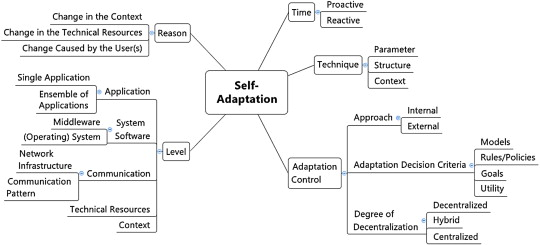
\includegraphics[width=\textwidth]{images/KrupitzerTaxonomy.jpg}
    \caption{Taxonomy for \acrshort{sas} \cite*{SurveyOnEngineeringApproaches}}
    \label{fig:KrupitzerTaxonomy}
\end{figure*}

\noindent The taxonomy for \acrshort{sas} in Figure \ref{fig:KrupitzerTaxonomy}
is based upon the 5W+1H questions by Salehie and Tahvildari \cite*{LandscapeAndResearchChallenges}.
These questions are: Where, When, What, Why, Who and How.
Each of these questions is responsible for a different aspect of \acrshort{sas} and corresponds to a dimension of the taxonomy.

\subparagraph*{Why}
First there needs to be a reason for a \acrshort{sas} to adapt. Why an adaptation should be performed is answered by the Reason dimension.
According to the taxonomy reasons for an adaptation can be changes in either the context, a technical resource or changes caused by the user.

\subparagraph*{Where}
The question of where asks on which level of the system changes need to occur.
The different levels on which changes can occur include:
\begin{itemize}[nosep]
    \item Different levels of applications from the operating system to a user application
    \item How systems communicate with each other
    \item The technical resources that are needed by the system
    \item The context in which the system operates
\end{itemize}

\subparagraph*{When}
While the original When-Question by Salehie and Tahvildari tries to understand all temporal aspects of \acrshort{sas},
including how frequently changes should occur and if they happen continously,
the taxonomy only answers the question when changes should be performed.
For this purpose the Time dimension differentiates between systems that perform changes proactively or reactively.
Reactive changes occur after, for example, a system metric has been violated.
Proactive changes occur before a system metric can be violated.

\subparagraph*{What}
In addition to the question of where and when changes should occur, it is also important to know
what changes should occur. There are different techniques that can be used.
The Technique dimension of the taxonomy differentiates between systems that change parameters, their structure or their context.
A system that changes its structure could, for example, be a datacenter, which starts new server instances on demand.
Robots are an example for systems that change their context.
This is achieved by, for example, moving the robot around.

\subparagraph*{Who}
After answering where, when, what and why changes should be performed, 
it is necessary to select who is responsible for these changes.
According to Salehie and Tahvildari it is also important to establish if the changes can be performed fully autonomous
or if the involvement of human operators is necessary.
The taxonomy does not directly address all of these concerns but states that:
"N/A (nature of a SAS leads to an automatic type of adaptation)" \cite{SurveyOnEngineeringApproaches}.

\subparagraph*{How}
Lastly, after determining the where, when, what, why and who, there needs to be a way
to perform the required changes. This is answered by asking how the changes should be performed
and corresponds to the Adaptation Control.
The three main aspects of the Adaptation Control are the degree of decentralization, the adaptation decision criteria
and the approach taken by the system.
The degree of decentralization ranges from systems which perform adaptations through a central component (fully centralized)
to systems where each component is responsible for its own adaptation (fully decentralized).
In between these two degrees are systems that employ a hybrid approach.
The adaptation decision criteria controls how the adaptation is achieved.
Krupitzer et al. propose the following possibilities:
\begin{itemize}[nosep]
    \item Models: The \acrshort{sas} updates e.g. domain models which results in behavioral changes
    \item Rules/Policies: The \acrshort{sas} changes its behavior based on rules or policies
    \item Goals: The \acrshort{sas} changes its behavior to meet some predefined set of goals
    \item Utility: The \acrshort{sas} changes its behavior to maximize or minimize a utility function
\end{itemize}
The approach divides \acrshort{sas} into those where the adaptation logic is part of the application logic
and those with separated adaptation and application logic.

\noindent After classifying \acrshort{sas} the following question can be asked: Which parts of a \acrshort{sas} can be optimized?
To answer this we will start by looking at which parts can not be optimized or do not benefit from optimization.

\noindent The first part that can not be optimized is the environment which provides the Reason dimension.
While the environment for a \acrshort{sas} can be chosen in a way which is most beneficial for the system
and can be influenced by actors,
the behavior of the systems environment can generally not be controlled.

\noindent Another dimension of \acrshort{sas} that can not be optimized, or is not useful to optimize,
is the Time dimension. This dimension is mostly a design decision on how the system should behave and be constructed.
It is also a question of how to handle uncertainty and the level of accepted risk.
A proactive system can prevent faults and degradation in Quality-of-Service metrics,
but it can also predict the wrong changes which can lead to a situation where the system itself generates faults by
reacting in a way that is contradictive to its goals.
A reactive system can not prevent faults like a proactive system,
but its behavior can be much more stable, because it only has to react to a change and not predict that change as well.

\noindent Lastly, the question of who is responsible can not be optimized, because the taxonomy simply answers it,
by referring to the name "\acrshort{sas}" which implies that the system itself is responsible for managing adaptations.

\noindent The three remaining dimensions can be optimized or can benefit from being adapted dynamically.
These are the Adaptation Control, the Level and the Technique.

\noindent The Approach and the Degree of Decentralization used by the Adaptation Control can not be optimized 
because they are design decisions of how the system is built.
However, the Adaptation Decision Criteria can be optimized. An optimization of the Adaptation Decision Criteria
could, for example, be to dynamically adapt the rules and policies at runtime to better reflect a changing environment.

\noindent Another dimension that can be optimized is the Technique. 
This can be optimized by changing what gets adapted by the system.

\noindent The last dimension that can be optimized is the Level, which can be done by dynamically changing at which level of the system
adaptations should be performed.